% This is a basic Math Paper

\documentclass[11pt]{article}

% Preamble

\usepackage[margin=1in]{geometry}
\usepackage{amsfonts, amsmath, amssymb}
\usepackage{gensymb}
\usepackage{fancyhdr, float, graphicx}
\usepackage[utf8]{inputenc} % Required for inputting international characters
\usepackage[T1]{fontenc} % Output font encoding for international characters
\usepackage{fouriernc} % Use the New Century Schoolbook font
\usepackage[nottoc, notlot, notlof]{tocbibind}


% Header and Footer
\pagestyle{fancy}
\fancyhead{}
\fancyfoot{}
\fancyhead[L]{\textit{\Large{Engineering Mechanics Experiment 9}}}
%\fancyhead[R]{\textit{something}}
\fancyfoot[C]{\thepage}
\renewcommand{\footrulewidth}{1pt}



% Other Doc Editing
% \parindent 0ex
%\renewcommand{\baselinestretch}{1.5}

\begin{document}
	
	\begin{titlepage} 
		\centering 
		
		%---------------------------NAMES-------------------------------
		
		\huge\textsc{
			MIT World Peace University
		}\\
	
		\vspace{0.75\baselineskip} % space after Uni Name
		
		\LARGE{
			Engineering Mechanics\\
			First Year B. Tech, Trimester 1
		}
	
		
		\vfill % space after Sub Name
		
		%--------------------------TITLE-------------------------------
		
		\rule{\textwidth}{1.6pt}\vspace*{-\baselineskip}\vspace*{2pt}
		\rule{\textwidth}{0.6pt}
		\vspace{0.75\baselineskip} % Whitespace above the title
		
		
		
		\huge{\textsc{
				Graphical Solution of Problems involving Relative Motion between Two Bodies
			}} \\
		
		
		
		\vspace{0.5\baselineskip} % Whitespace below the title
		\rule{\textwidth}{0.6pt}\vspace*{-\baselineskip}\vspace*{2.8pt}
		\rule{\textwidth}{1.6pt}
		
		\vspace{1\baselineskip} % Whitespace after the title block

		%--------------------------SUBTITLE --------------------------	
			
		\LARGE\textsc{
			Experiment 11\\
			Practical Report
		} % Subtitle or further description
		\vfill
		
		%--------------------------AUTHOR-------------------------------
		
		Prepared By
		\vspace{0.5\baselineskip} % Whitespace before the editors
		
		\Large{
			Krishnaraj Thadesar \\
			Division 9, Roll No. 54
		}
		
		
		\vspace{0.5\baselineskip} % Whitespace below the editor list
		\today

	\end{titlepage}
	
	
\tableofcontents
\thispagestyle{empty}
\clearpage


\setcounter{page}{1}

\section{Objective}
To find Graphically the resultant of a set of problems involving relative motion between two bodies. 

\section{Theory}
The Following laws and concepts have been used in this experiment.

\subsection{Relative Velocity}
We encounter occasions where one or more objects move in a frame which is non-stationary with respect to another observer. For example, a boat crosses a river that is flowing at some rate or an aeroplane encountering wind during its motion. In all such instances, in order to describe the complete motion of the object, we need to consider the effect that the medium is causing on the object. While doing so, we calculate the relative velocity of the object considering the velocity of the particle as well as the velocity of the medium. Here, we will learn how to calculate the relative velocity.

Let us consider two objects, $A$ and $B$ moving with velocities $V_{a}$ and $V_{b}$ with respect to a common stationary frame of reference, say the ground, a bridge or a fixed platform.
The velocity of the object A relative to the object B can be given as,
$$
V_{a b}=V_{a}-V_{b}
$$
Similarly, the velocity of the object B relative to that of object a is given by,
$$
V_{b a}=V_{b}-V_{a}
$$
From the above two expressions, we can see that
$$
V_{a b}=-V_{b a}
$$
Although the magnitude of both the relative velocities is equal to each other. Mathematically, $$\left|V_{a b}\right|=\left|V_{b a}\right|$$

\begin{figure}[H]
	\centering
	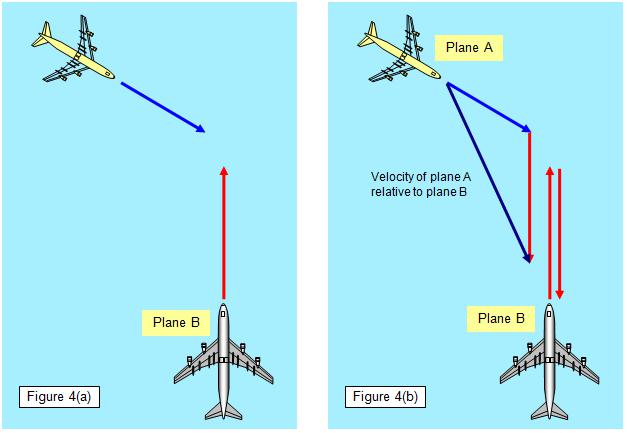
\includegraphics[scale=0.45]{rel vel.jpg}
	\label{fig: Polygon Law}
	\caption{Example of Relative Velocity}
\end{figure}


\pagebreak
\section{Graphical Method}

Q1. Two chips 'A' and 'B' are at a given instant 4 km  away from each other and both are on south east line. Ship 'A' is travelling at 8 km/hr due east and ship 'B' is travelling at 12 km/hr due north. Determine - \\
1. Velocity of 'B' with Respect to 'A'\\
2. The Shortest distance between the two ships. \\
3. Time to get to the shortest distance. \\

\begin{figure}[H]
	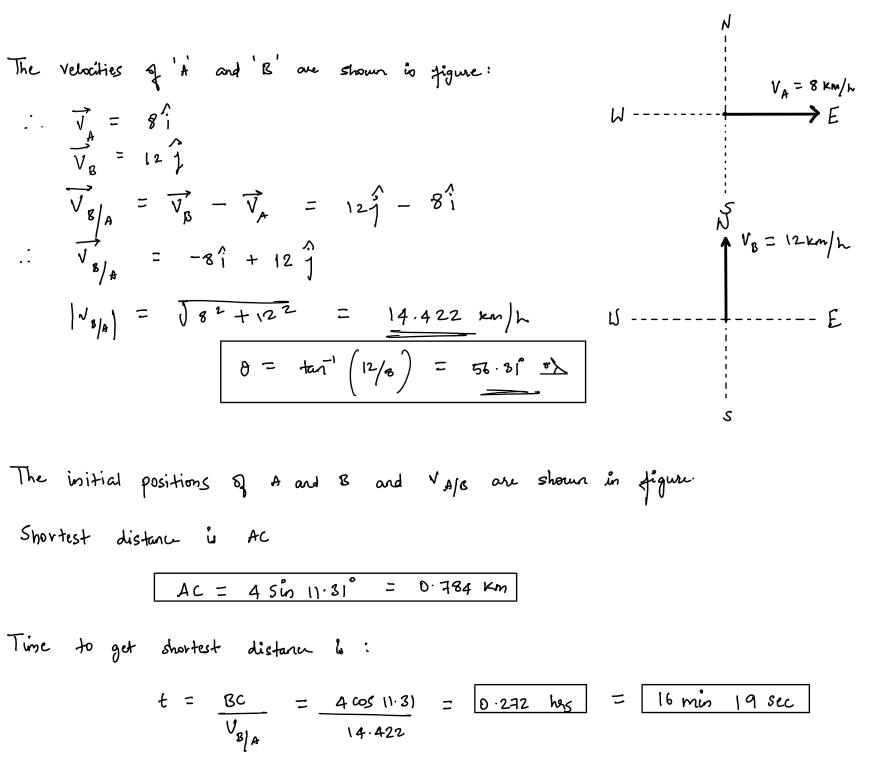
\includegraphics[scale=0.6]{g1.jpg}
	\label{fig: Polygon Law}
\end{figure}


\pagebreak
Q2. Two Planes A and B are flying at the same altitude. If their velocities are $ v_A = 600\ kmph $ and $ v_b = 500\ kmph $ and the angle between their straight courses is $ 75 \degree $, determine the velocity of plane B with respect to plane A and the shortest distance between them. 


\begin{figure}[H]
	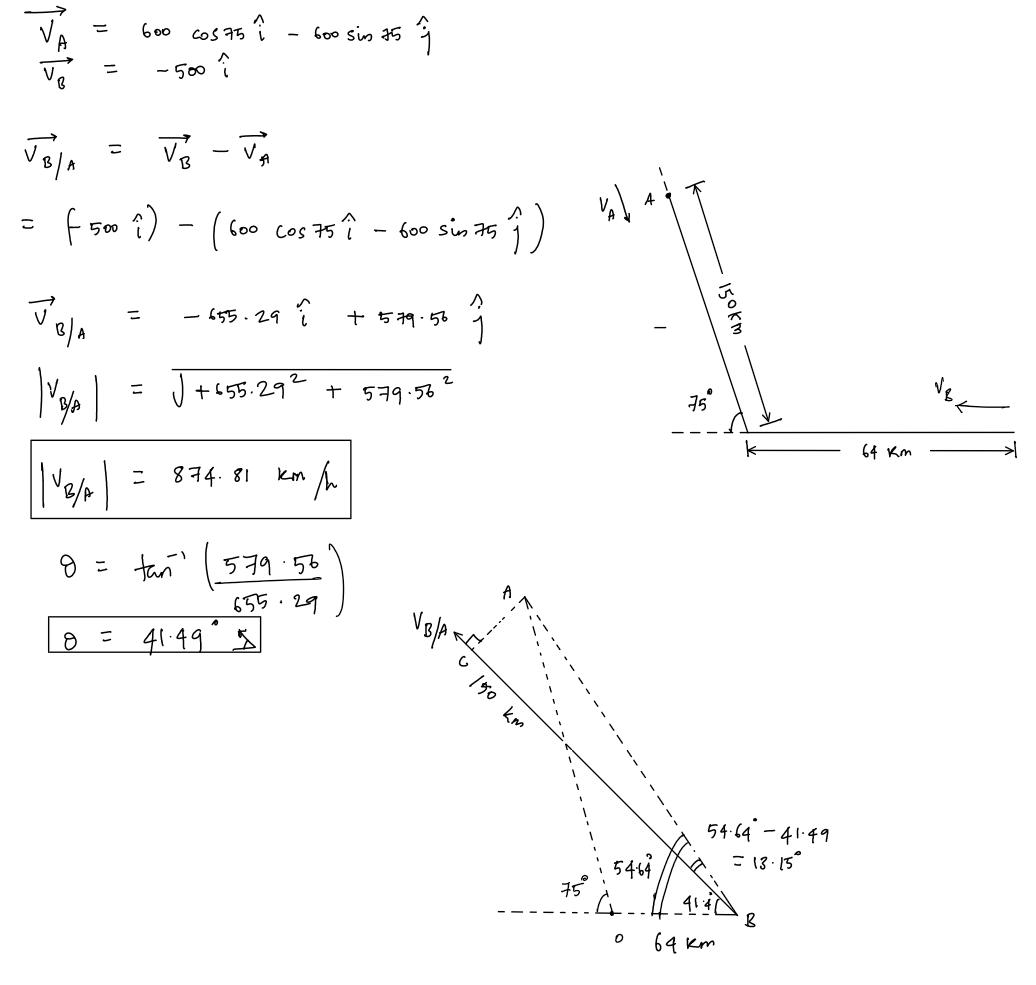
\includegraphics[scale=0.5]{g222.jpg}
	\label{fig: Polygon Law}
\end{figure}


\begin{figure}[H]
	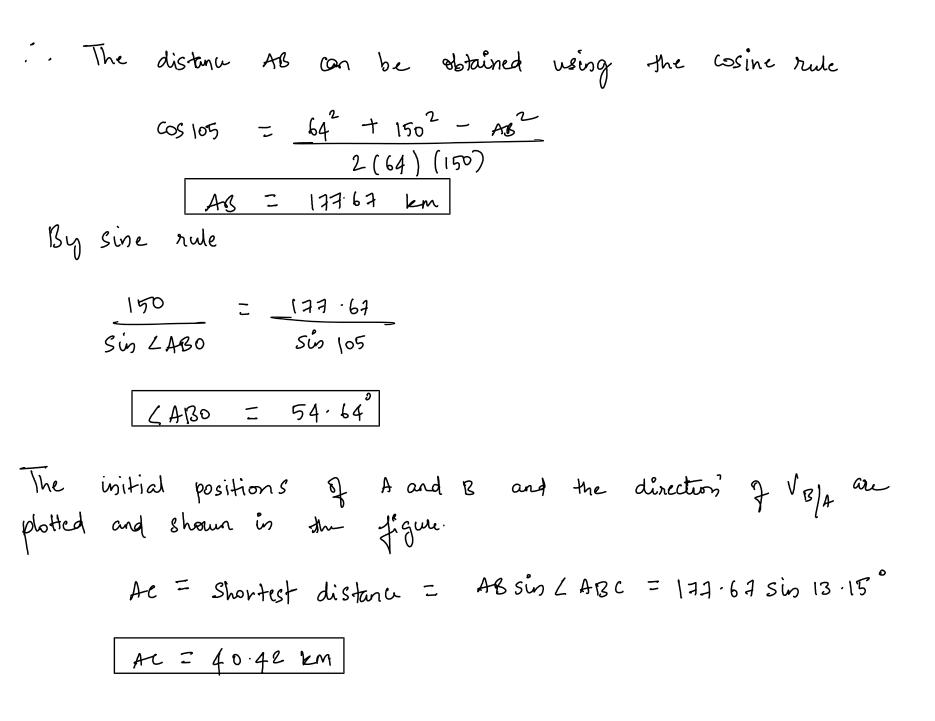
\includegraphics[scale=0.5]{g22.jpg}
	\label{fig: Polygon Law}
\end{figure}

\pagebreak

Q3. At an instant ship A is streaming due East at $  20 km/h $ and ship B at that instant is $ 80 km $ due South and is streaming at $ 16 km/h $. Determine: \\
1. $ v_{B/A} $\\
2. Shortest distance between them.\\
3. time to attain the shortest distance.

\begin{figure}[H]
	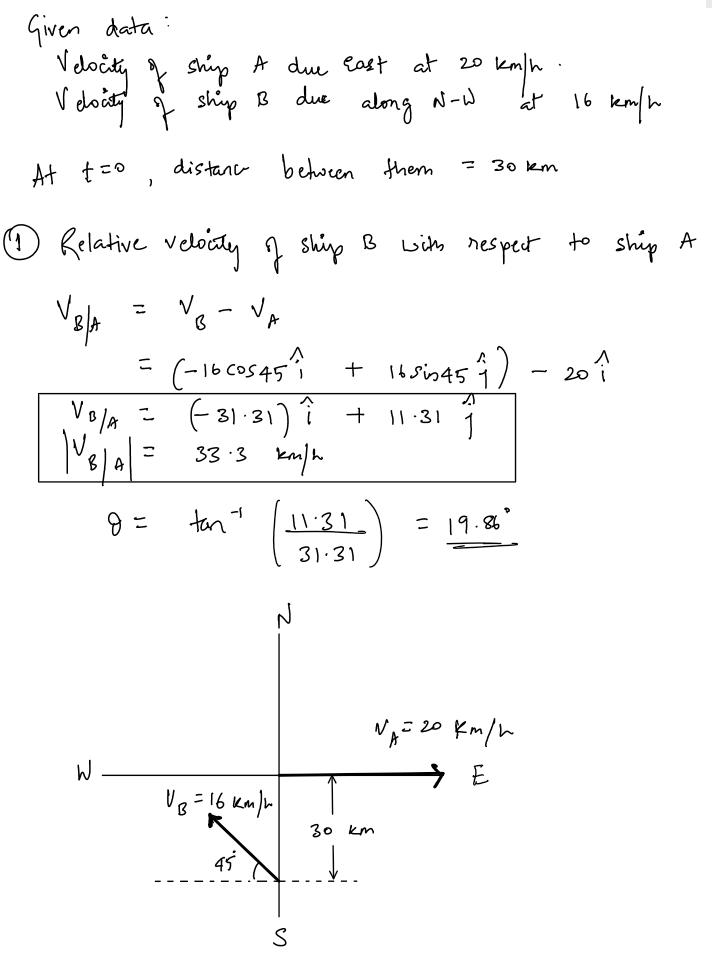
\includegraphics[scale=0.55]{g31.jpg}
	\label{fig: Polygon Law}
\end{figure}

\begin{figure}[H]
	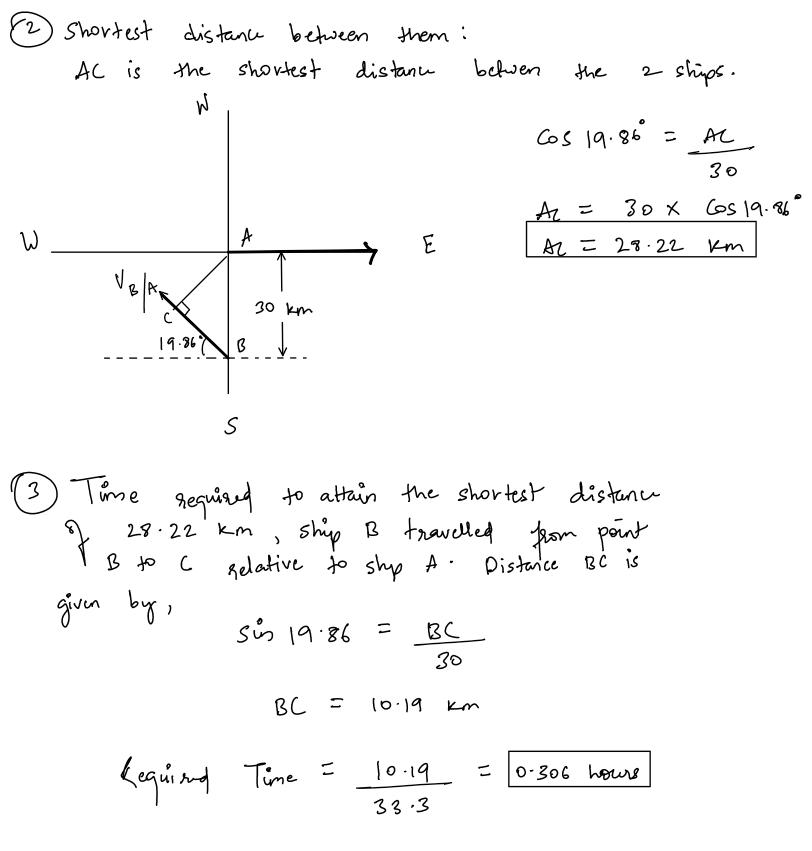
\includegraphics[scale=0.6]{g32.jpg}
	\label{fig: Polygon Law}
\end{figure}
\pagebreak

\section{Conclusion}
A set of problems involving involving relative motion between two bodies were solved using graphical method.
\end{document}